Next, we constructed the two-way current divider shown in Figure \ref{fig:exp3circuit2}, such that the divider ratio was
a small integer multiple. We measured the output current as we swept the input current, fitting a straight line to the data collected.


\begin{figure}[H]
\centering
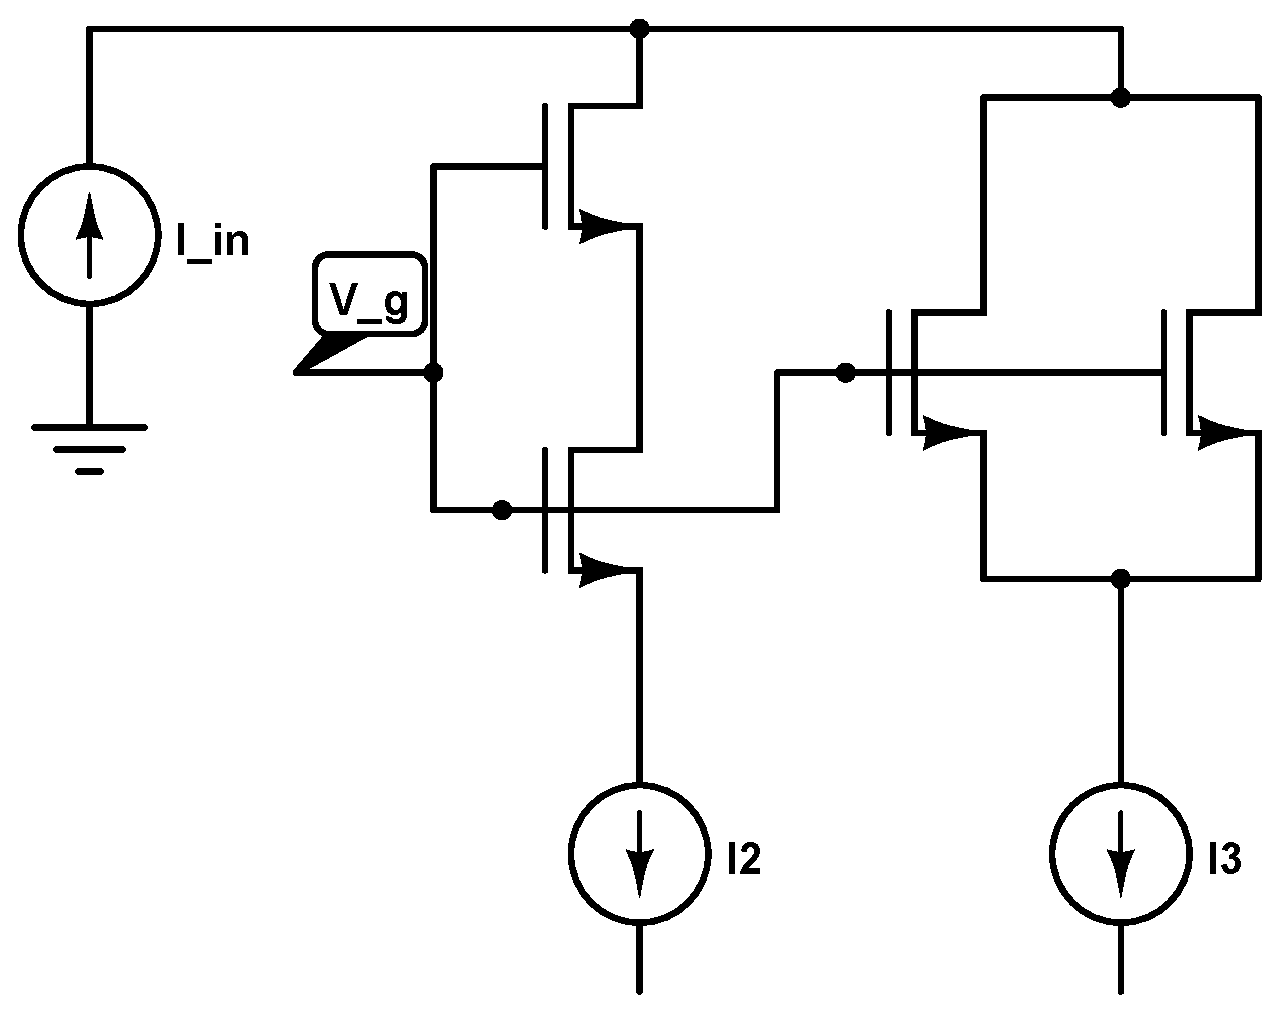
\includegraphics[width=0.55\linewidth]{../Figures/Experiment3CircuitDiagram2.eps}
\caption{A diagram of the circuit used in Experiment 3 Section 2}
\label{fig:exp3circuit2}
\end{figure}


As can be seen in Figure \ref{fig:exp3fit2}, the data fit a straight line well, with an extracted slope of $0.80298$. Drawing upon our previous knowledge from Experiment 2, where we found that the series combination of two \nMOS transistors passed half the current as a single \nMOS, and the parallel combination passed twice the current of a single \nMOS, we can infer that the series combination passed one quarter the current of a parallel combination. 
Thus, for a given set of voltages, \Vg, \Vd, \Vb, \Vd and \Vs, we expect the theoretical ratio of current passed to be 1:4 between the series and parallel combinations, respectively. A 1:4 ratio is the same as a fifth of the current being passed through the series combination, and four-fifths of the current through the parallel combination. As seen in Figure \ref{fig:exp3fit2}, the extract slope was almost exactly $4/5$ or $0.8$.

\begin{figure}[H]
\centering
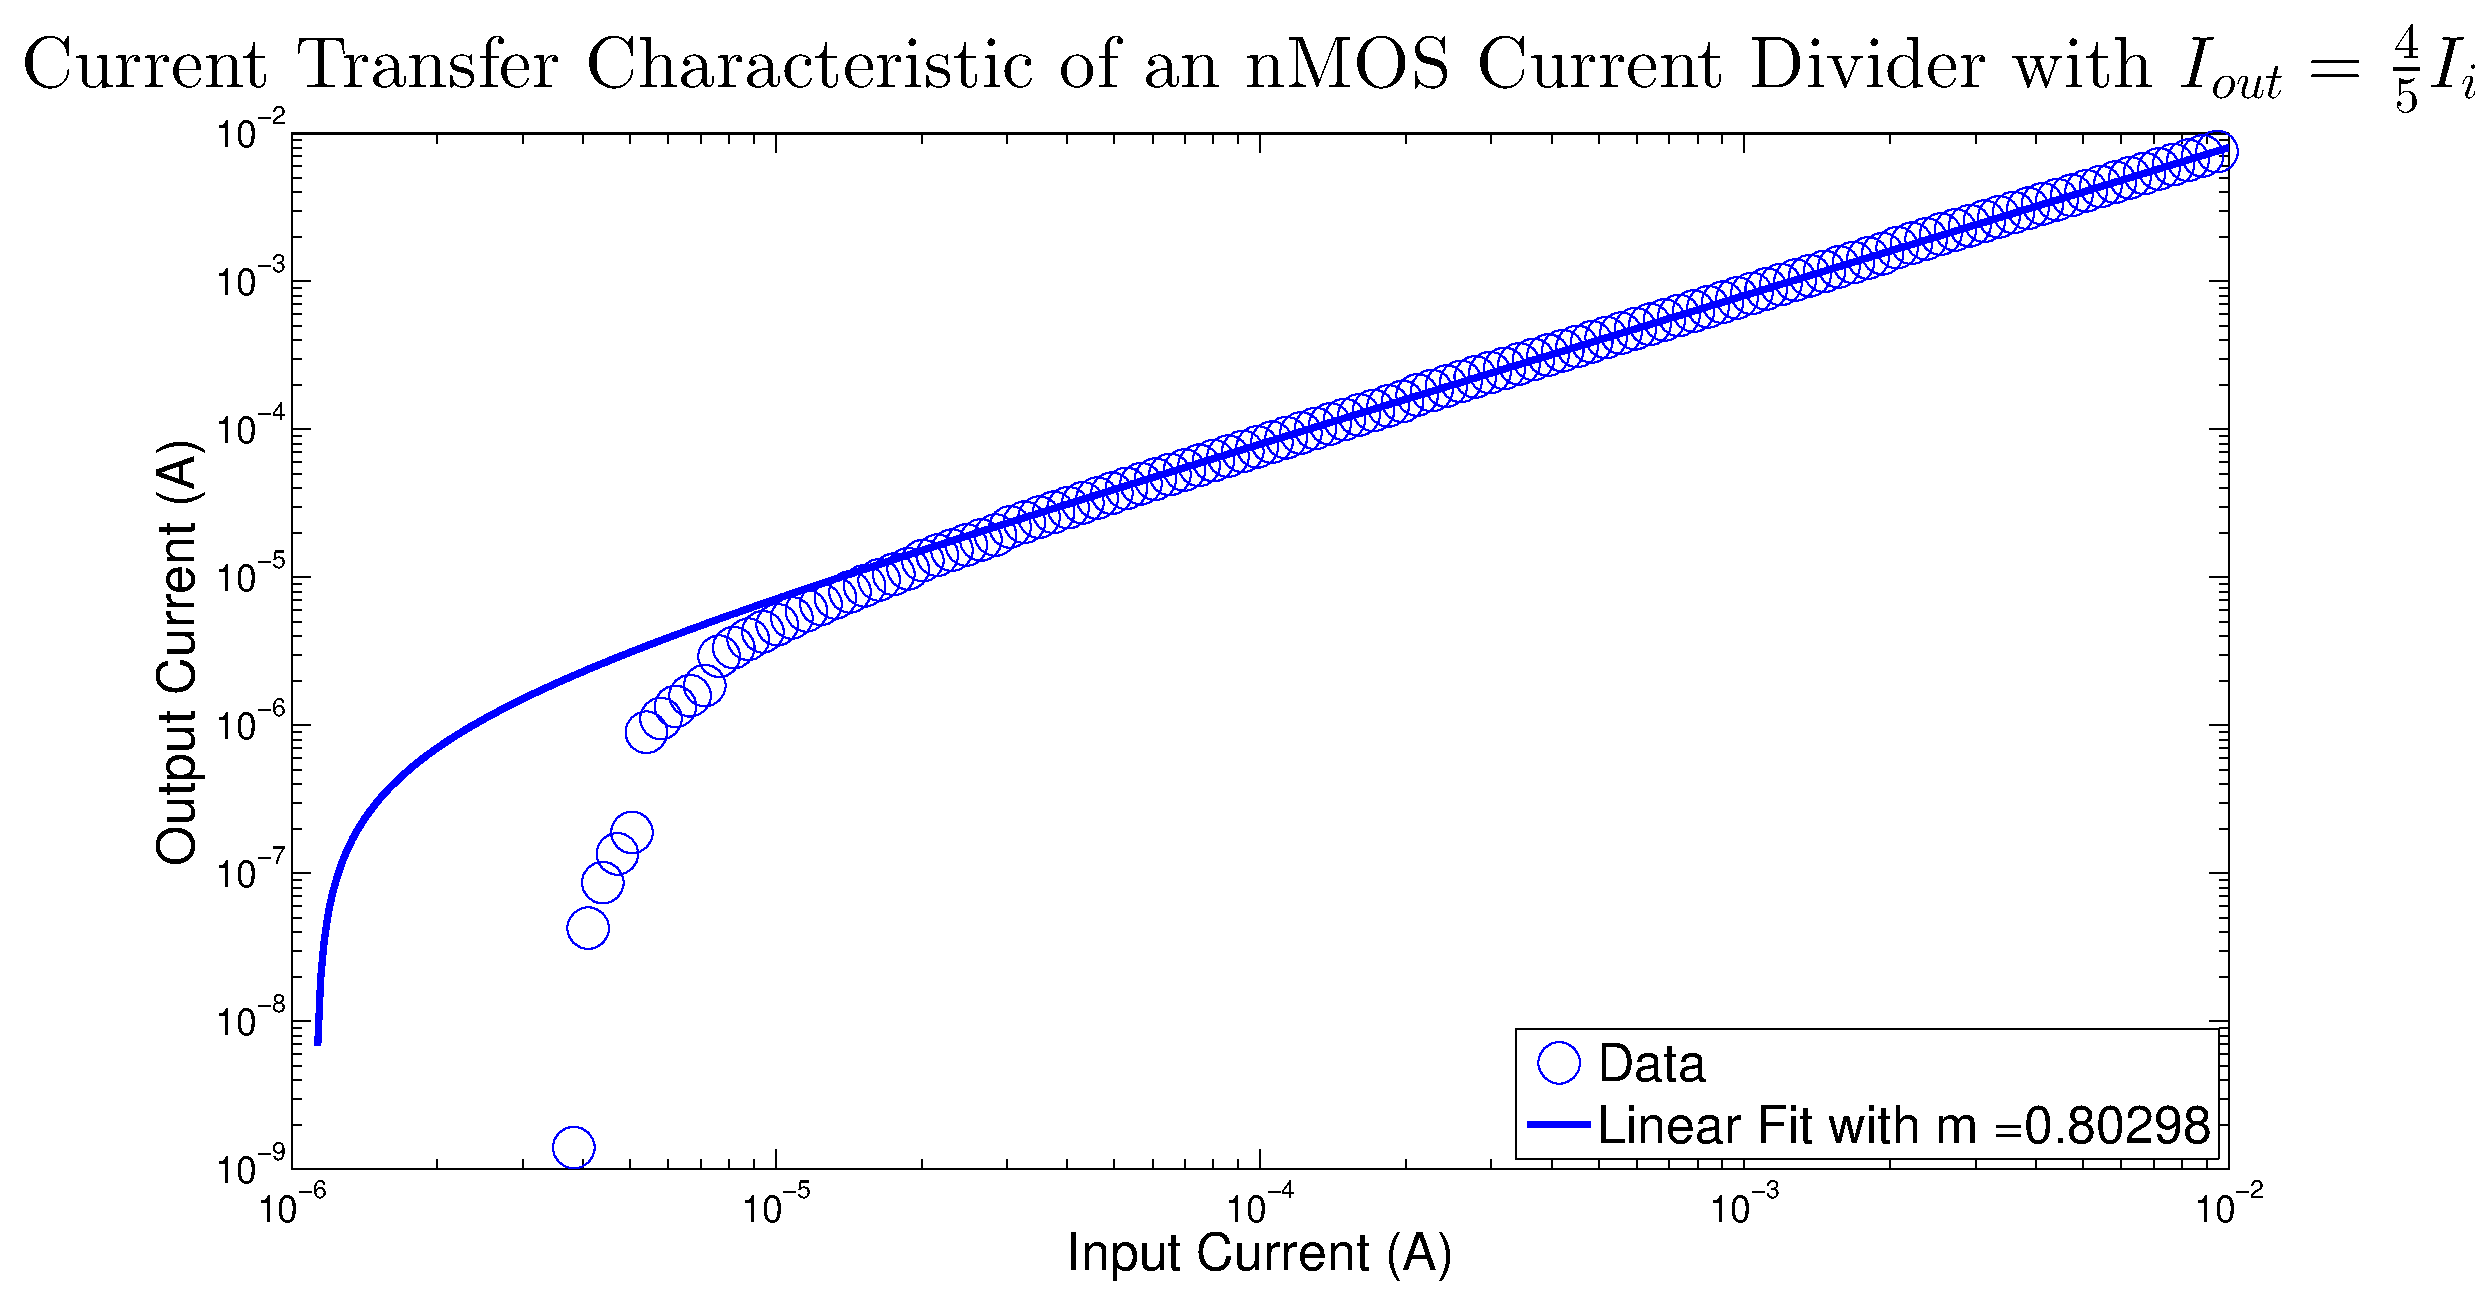
\includegraphics[width=\linewidth]{../Figures/Experiment3Figure2.eps}
\caption{A plot of the current through the parallel combinaton of \nMOS, as a function of input current.}
\label{fig:exp3fit2}
\end{figure}

To explain the difference between the two current divider circuits, we need to understand how $V_{DS}$ changes for both circuits as we increase \Iin. In the case where we pull current from the sources of both branches, small currents will induce a small source voltage, which will be more than $V_{DSSat}$ away from \Vdd, ensuring that both branches will remain in saturation. In the second circuit, where we push \Iin through the drains of both branches, we see that the circuit only begins operating as we expect it to once we pass a certain current threshold. This can be explained by examining the drain voltage for small values of \Iin. When \Iin is small, we expect the drain voltage to be small, as only a small amount of current passes through the branch of each transistor. The branch of the current divider with the series transistors requires that the input voltage be at least $2V_{DSSat}$, as both transistors need to be in saturation for proper circuit operation. This minimum voltage threshold is the analog to the minimum current threshold we saw in figure \ref{fig:exp3fit2}, and explains why the circuit in figure \ref{fig:exp3p1dia} is a better current divider circuit compared to the circuit in figure \ref{fig:exp3circuit2}.
